\documentclass[12pt,letterpaper]{article}
\usepackage[margin=1in]{geometry}
\usepackage{fancyhdr}
\usepackage[utf8]{inputenc}
\usepackage{palatino}
\usepackage{microtype}
\usepackage{hyperref}
\usepackage{graphicx}
\usepackage{lastpage}
\usepackage[hang,small]{caption}
\usepackage{titlesec}
\usepackage{amsmath,amssymb}
\usepackage{multirow}

\renewcommand{\headrulewidth}{0pt}
\fancyfoot{}
\fancyfoot[C]{\sf Page \thepage\ of \pageref{LastPage}}
\pagestyle{fancy}

\titleformat{\section}{\bfseries\Large}{\arabic{\thesection}}{1em}{}
\titleformat{\subsection}{\bfseries\large}{\arabic{\thesection}.\arabic{\thesubsection}}{1em}{}
\titleformat{\subsubsection}{\itshape}{\arabic{\thesection}.\arabic{\thesubsection}.\arabic{\thesubsubsection}}{1em}{}

\setlength{\parindent}{0cm}
\setlength{\parskip}{0.8em}

\captionsetup[figure]{labelfont=it,font=it}
\captionsetup[table]{labelfont={it,sc},font={it,sc}}

\hypersetup{colorlinks,
  linkcolor = black,
  citecolor = black,
  urlcolor  = black}
\urlstyle{same}



\begin{document}

Soo-Hyun Yoo \\
ST314 \\
Data Analysis 3 \\
November 4, 2014

\begin{enumerate}
  \item
    \begin{enumerate}
      \item \hfill\\
        \begin{table}[!h]
          \centering
          \begin{tabular}{|c|c|c|c|c|c|c|c|} \hline
            Min & 1st Qu. & Median & Mean & 3rd Qu. & Max. & $\sigma$ \\ \hline
            23.90 & 27.60 & 28.85 & 28.87 & 30.32 & 33.20 & 2.0886 \\ \hline
          \end{tabular}
        \end{table}

      \item \hfill\\ 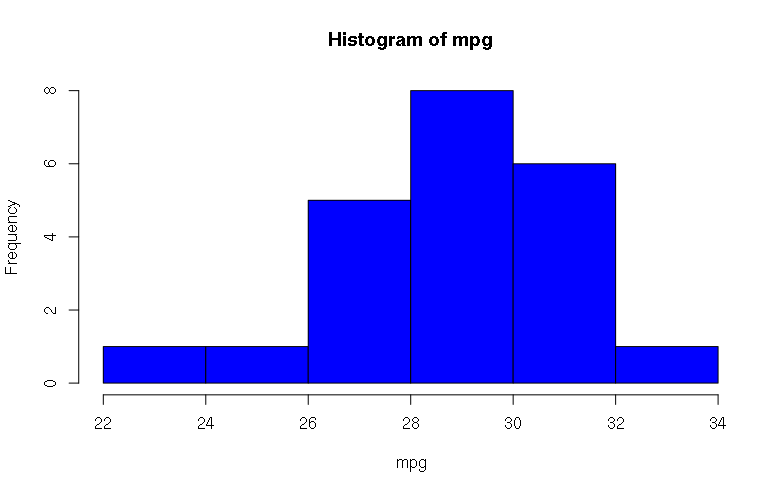
\includegraphics[width=0.8\textwidth]{1b.png}

        The true mean appears to be slightly less than 30 mpg.

      \item $H_0: \mu = 30$

        $H_a: \mu < 30$

      \item The histogram is not heavily skewed, so it may be reasonable to
        think the population distribution is normally distributed. However, the
        number of samples is fewer than 30, so we must use a t test.

      \item $t = \cfrac{\bar{X} - \mu}{\frac{s}{\sqrt{n}}} = \cfrac{28.87 - 30}{\frac{2.0886}{\sqrt{22}}} = \boxed{-2.5377}$

        p-value is $cdf(-2.5377, 21) = \boxed{0.00957}$

      \item $CI = \bar{X} \pm t_{0.05,21}\frac{s}{\sqrt{n}} = 28.87 \pm -1.7207 \cdot \frac{2.0886}{\sqrt{22}} = \boxed{(28.10, 29.64)}$

      \item R gives $t = -2.5417$, $df = 21$, p-value $= 0.009491$, and
        a confidence interval of $(-\infty, 29.63442)$. These numbers are
        slightly different from the hand calculations, probably due to rounding
        errors. The confidence interval's lower bound of $-\infty$ is likely
        due to the very low p-value; including the rest of the left tail does
        not significantly add to the ``95\%''

      \item There is convincing evidence that the average mileage is less than
        the claimed 30 mpg. The 95\% confidence interval estimates the average
        mileage to be at most 29.634 mpg, with a point estimate of 28.87 mpg.
        We reject the null with a one-sided p-value of 0.0095 at the 0.05
        significance level.

      \item
        \begin{verbatim}
a) mpg  = c(23.9, 28.4, 25.8, 33.2, 31.1, 30.4, 29.8, 27.6,
            29.0, 29.7, 31.1, 30.4, 28.7, 26.9, 27.5, 28.4,
            30.7, 30.1, 28.7, 26.2, 27.6, 29.9)
   summary(mpg)
   sd(mpg)
   hist(mpg, col="blue")
f) t.test(mpg, mu = 30, alternative = "less")
        \end{verbatim}
    \end{enumerate}

  \item
    \begin{enumerate}
      \item Whether or not the proportion of students enrolled at the college
        that binge drink is greater than the national proportion.

      \item $H_0: p = 0.401$

        $H_a: p > 0.401$

      \item The sample was obtained using a random mechanism and the sample
        size is large ($n>30$). However, the population standard deviation is
        {\bf not} known.

      \item $z = \cfrac{\hat{p} - p_0}{\sqrt{p_0(1-p_0)/n}} = \cfrac{\frac{231}{502} - 0.401}{\sqrt{0.401(1-0.401)/502}} = \boxed{2.7045}$

      \item One sided p-value: $1-cdf(2.7045) = \boxed{0.0034}$

      \item $CI = \hat{p} \pm z_{0.90}\sqrt{\frac{\hat{p}(1-\hat{p})}{n}} = 0.460 \pm 1.2816\sqrt{\frac{0.460(1-0.460)}{502}} = \boxed{(0.432, 0.489)}$

      \item There is convincing evidence that the proportion of students at
        this college that binge drink is greater than the national proportion
        of 0.401. The 90\% confidence interval estimates the proportion to be
        between 0.432 and 0.489, with a point estimate of 0.460. We reject the
        null with a one-sided p-value of 0.0034 at the 0.10 significance level.
    \end{enumerate}

  \item
    \begin{enumerate}
      \item The rejection region approach allows us to determine explicitly
        whether or not to reject the hypothesis. The p-value approach adds to
        this in that we can determine how convincingly we can reject or fail to
        reject the hypothesis.

      \item A sample size of 5 is not large enough to allow us to assume the
        distribution is normal. The skewedness of the distribution also may
        suggest it is not a normal distribution, which means we must choose the
        median or mode as the sample average.
    \end{enumerate}
\end{enumerate}

\end{document}

